% =============================================================================
% Section 5.2.3: End-to-End Testing
% =============================================================================

\subsection{End-to-End Testing}
\label{sec:e2e-testing}

End-to-end (E2E) tests exercise complete user-facing workflows through the HTTP API, validating that all layers---controller, service, repository, database, and external provider integration---operate correctly as an integrated system. E2E tests bootstrap the full NestJS application with all modules loaded, connect to Testcontainer-managed PostgreSQL and Redis instances, and interact exclusively through the public REST endpoints.

\subsubsection{E2E Test Organisation}

E2E tests are organised by user role and primary use case, following the user-story format established in Chapter~1. Table~\ref{tab:e2e-scenarios} lists the key E2E scenarios and the test files that implement them.

\begin{table}[H]
  \centering
  \caption{End-to-End Test Scenarios}\label{tab:e2e-scenarios}
  \small
  \begin{tabular}{lll}
    \toprule
    \textbf{Test File}                       & \textbf{Role}   & \textbf{Scenario} \\
    \midrule
    \texttt{auth.e2e-spec.ts}                & Student         & Register, verify email, login, refresh, logout \\
    \texttt{courses.e2e-spec.ts}             & Instructor      & Create course, add module, add lessons, publish, preview \\
    \texttt{assessment.e2e-spec.ts}          & Student         & View quiz, submit answers, receive grade, review feedback \\
    \texttt{media.e2e-spec.ts}               & Instructor      & Upload video, await transcoding, verify HLS stream URL \\
    \texttt{payment.e2e-spec.ts}             & Student         & Select course, create payment intent, complete checkout \\
    \texttt{enrollment.e2e-spec.ts}          & Student         & Enrol in course, access lesson, update progress, complete \\
    \texttt{discussion.e2e-spec.ts}          & Student         & Create thread, post reply, moderate by instructor \\
    \texttt{reviews.e2e-spec.ts}             & Student         & Submit review, update rating, verify eligibility rules \\
    \texttt{ai-pipeline.e2e-spec.ts}         & Instructor      & Submit video for AI processing, await quiz generation \\
    \midrule
    \textbf{Total: 9 files, 34 test cases}  & (3 roles)       & (9 complete workflows) \\
    \bottomrule
  \end{tabular}
\end{table}

\subsubsection{Representative E2E Flow: Student Enrollment}

The student enrollment flow (Figure~\ref{fig:e2e-enrollment}) spans three bounded contexts---Auth, Payment, and Enrollment---and five HTTP endpoints. The E2E test executes the following sequence:

\begin{enumerate}
  \item \texttt{POST /auth/register} --- Create a new student account. Assert HTTP 201 with activation token in response body.
  \item \texttt{POST /auth/verify-email} --- Submit the activation token. Assert HTTP 200 and a success message.
  \item \texttt{POST /auth/login} --- Authenticate with email and password. Assert HTTP 200, capture the access and refresh tokens from response headers.
  \item \texttt{GET /courses/:id} --- Fetch course details to confirm the course is published and priced. Assert HTTP 200 with course metadata including price.
  \item \texttt{POST /payments/create-intent} --- Create a Stripe PaymentIntent for the course price. Assert HTTP 201 with a \texttt{clientSecret} field.
  \item \texttt{POST /webhooks/stripe} --- Simulate Stripe's \texttt{payment\_intent.succeeded} webhook with HMAC signature. Assert HTTP 200.
  \item \texttt{GET /enrollments} --- Verify the enrollment record exists in \texttt{ACTIVE} state. Assert HTTP 200 with a non-empty array containing the enrollment.
  \item \texttt{GET /lessons/:id} --- Access a lesson to confirm the enrollment grant is respected. Assert HTTP 200 with lesson content.
\end{enumerate}

All assertions include HTTP status code verification, response body shape validation (using \texttt{expect.objectContaining} for partial matching), and database state verification via direct Prisma queries to confirm that side effects were persisted correctly.

\begin{figure}[H]
  \centering
  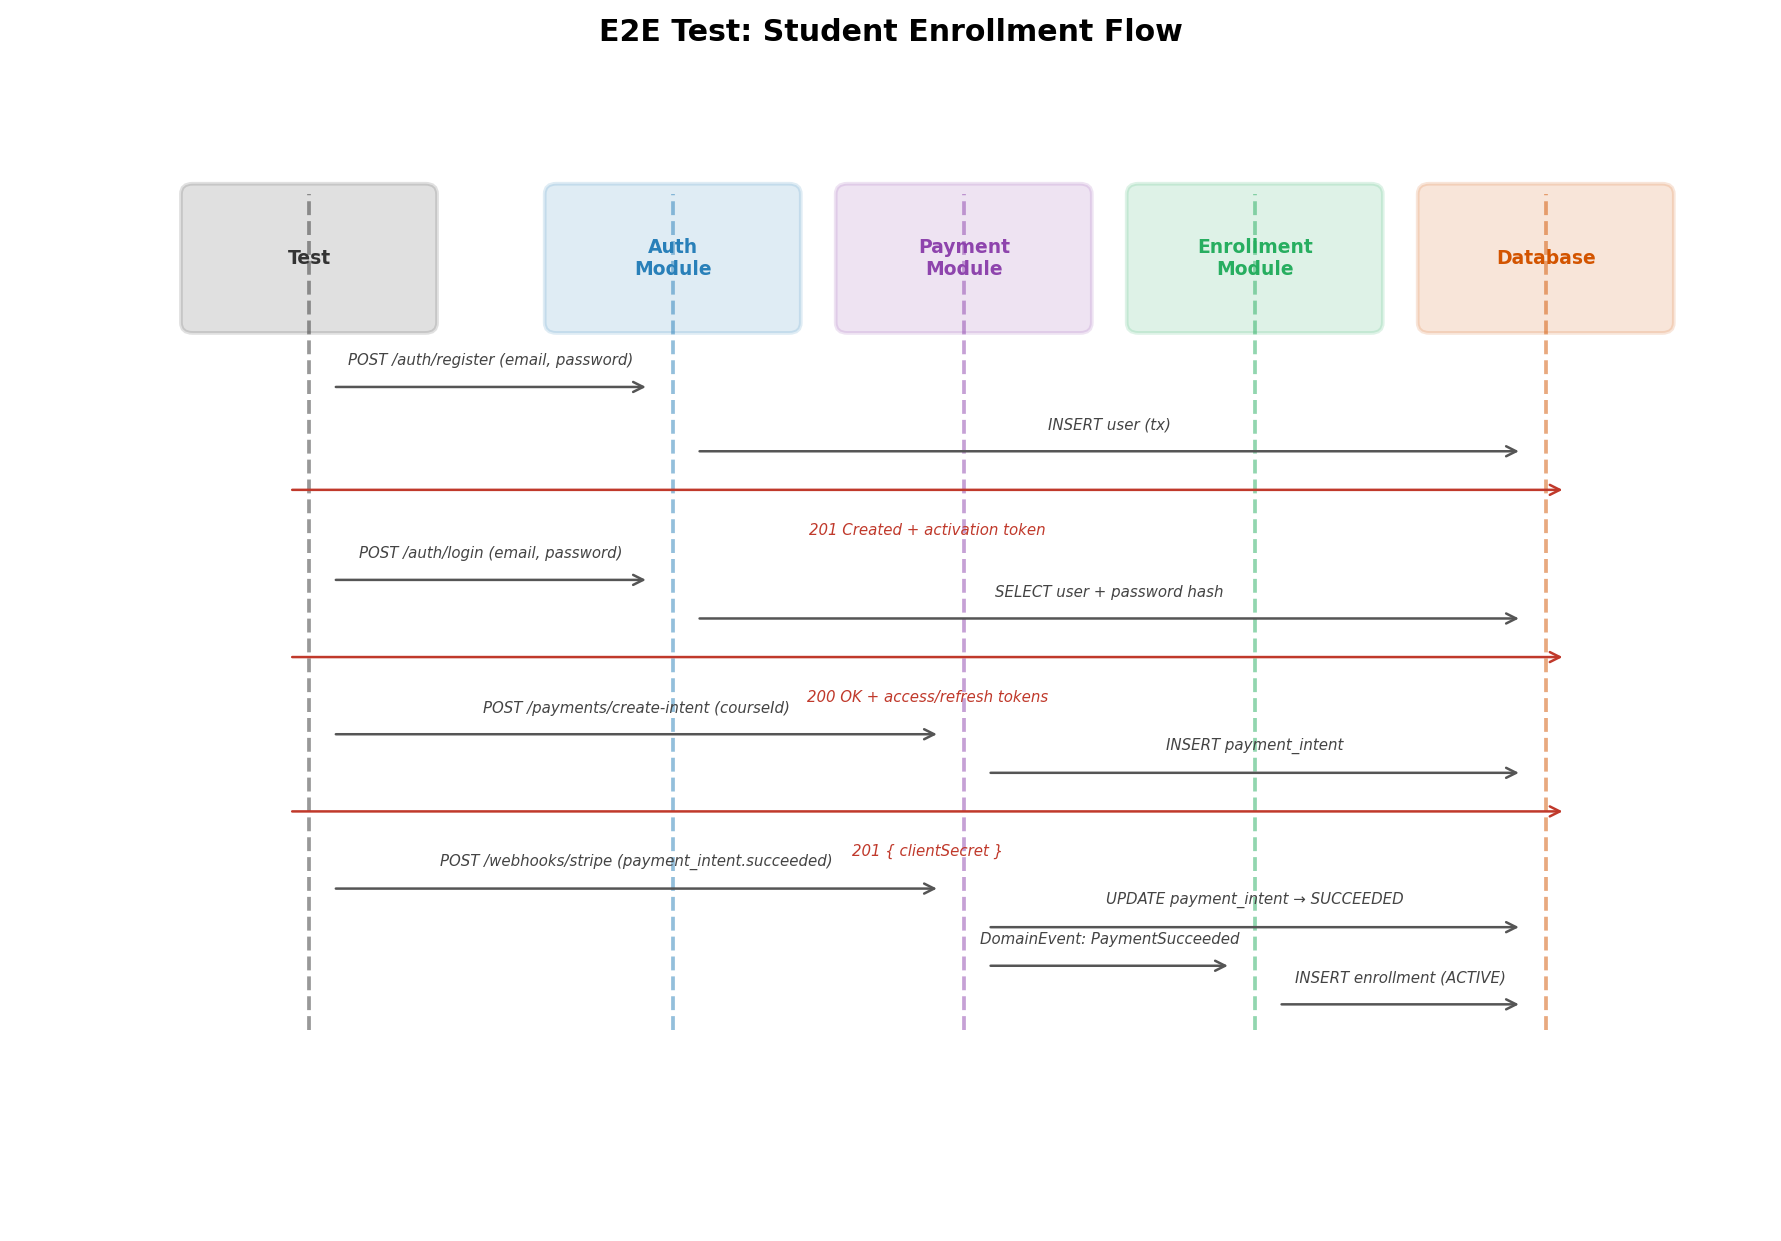
\includegraphics[width=0.85\textwidth]{images/e2e_enrollment_flow.png}
  \caption{E2E test sequence diagram for the student enrollment flow, showing HTTP calls across Auth, Payment, and Enrollment modules.}\label{fig:e2e-enrollment}
\end{figure}

\subsubsection{Instructor Quiz Creation and AI Pipeline}

A second critical E2E scenario validates the AI-powered quiz generation pipeline. The instructor uploads a video, waits for AI processing to complete (via a polling loop with a 30-second timeout), and verifies that a quiz has been automatically generated:

\begin{lstlisting}[caption=E2E test for AI quiz generation,label=lst:e2e-ai-quiz]
it('generates a quiz from an uploaded video', async () => {
  // Instructor logs in
  const instructor = await loginAs('instructor@test.edu', 'password123');
  const courseId = await createCourse(instructor.token, 'Test Course');
  const lessonId = await addLesson(instructor.token, courseId, 'Test Lesson');

  // Upload video
  const videoRes = await request
    .post(`/media/upload`)
    .set('Authorization', `Bearer ${instructor.token}`)
    .attach('file', Buffer.from('fake-video-content'), 'lecture.mp4');
  expect(videoRes.status).toBe(201);
  const videoAssetId = videoRes.body.id;

  // Attach video to lesson and request AI processing
  await request
    .post(`/courses/${courseId}/modules/${moduleId}/lessons/${lessonId}/video`)
    .set('Authorization', `Bearer ${instructor.token}`)
    .send({ videoAssetId, generateQuiz: true });

  // Poll for quiz generation completion (max 30 seconds)
  const quiz = await pollForQuiz(instructor.token, lessonId, 30_000);
  expect(quiz.questions.length).toBeGreaterThanOrEqual(3);
  expect(quiz.status).toBe('PUBLISHED');
});
\end{lstlisting}

This test was instrumental in identifying a race condition where the AI pipeline callback arrived before the database transaction that created the \texttt{QuizGenerationJob} record had committed, causing a foreign key violation. The fix involved reordering the transaction to upsert the job record before sending the callback acknowledgement.
